\chapter{Collusion}
\label{chap:Collusion}

In this chapter we consider what is informally called malware, how malware differs from useful software and confront the limitations to detecting malware.  We then introduce collusion as a special type of malware and give a formal description.

\section{Malware on Android}
The term `malware' is a portmanteau of malicious and software.  Malware is software that intentionally performs activities that are detrimental to the user, computer systems or networks.  The intentions are to cause harm, disruption, make a financial gain or steal information.  In short, we can associate this software with unlawful activity.  Malware must hide its real intention from the user and thus, will pose as benign software that offers some attractive service.  But unknown to the user, it will perform other functions that benefit the creator in ways the user has not consented to.\\

Android is one of the two most popular platforms for mobile devices.  In 2019 it was estimated there were 3.4 billion reported smartphone user's worldwide \cite{SmartphoneUsers2019}, and 1.6 billion were Android smartphones \cite{AndroidUsers2019}.  Malware is a real problem on Android, not just theorised, and can potentially affect all these users.  Just a selection of reports contain hundreds of malware examples discovered in the wild: \cite{GhimobMalware}, \cite{AlienMalware}, \cite{CryloggerInTheWild}.  Attacks happen to such an extent that the McAfee Q1 2020 threat report opens with the headline ``Mobile Malware Is Playing Hide and Steal'' \cite{McAfeeMobileThreatReport}.  The report goes on to describe the discovery of a variety of attacks and the latest techniques the authors are using to hide their malware.

On Android devices, malware can take many forms, including:

\begin{enumerate}
\item Information theft.  Where malware sends information on the device outside the device without the user's permission.  We class spyware as information theft.
\item Ransomware.  Where information or services are restricted until the user has met the demands of a malicious actor.
\item Monetary theft.  Where the activities of an application must be paid for financially by the user, such as an application sending SMS messages without the user's permission or responding to advertisements.
\item Controlling device services such as using the device to mine cryptocurrency without the user's knowledge.
\end{enumerate}

In this project, we focus specifically on information theft but, we see no reason why the techniques proposed here cannot be used to detect other types of malware.

\section{The Difference Between Malicious and Benign Software}

ISO27005 defines a security threat as: ``A potential cause of an incident, that may result in harm of systems and organisations.''

The challenge we face when detecting malicious software is that the actions performed during an attack also have harmless purposes.  For instance, many beneficial applications can view photos, and many applications communicate with each other to increase the features they offer.  The difference is one of intent.  Operating system calls used for benign purposes can also be put to use by malicious software to perform an attack.  The difference is that malware intends to benefit a malicious actor at the user's expense and without their knowledge.  But without a detailed specification of what the software intends to do, we cannot decide if the actions it performs are to benefit the user or a malicious actor.

The trouble with the Android case is that detailed specifications of applications do not exist. The official publisher of Android applications is the Google Play store.  The descriptions this repository provides are only brief and written by the developer.  Firstly, a malicious developer will not document their real intent, and secondly, the benign developer does not wish to bore the potential user with a technical specification.  For instance, the description of the AccuWeather app begins:\\

``From weather updates to today's temperature, get the accurate weather forecast you know you can rely on with AccuWeather. With in-depth forecast news, the latest forecast updates, severe weather alerts, today's weather, and much more. Our precision and scientific accuracy let you stay one step ahead of the daily forecast and is the weather tracker that makes the unpredictable, predictable.''\\

The description continues in this vein but says nothing about the user's privacy. The Play store does attempt to help the user further by providing reviews from other users. However, user reviews cannot be trusted because we know from the 2020 McAfee threat report \cite{McAfeeMobileThreatReport} that malware already exists with the ability to post fake reviews for other malware.

Without a documented objective, how can we tell if the actions performed are to achieve that objective or a hidden malicious objective?  We cannot tell.  We can only recognise behaviour patterns that suggest applications may be behaving in a threatening manner.  Once we identify a threat pattern, we have no other option but to make the pessimistic assumption that the applications are involved in malicious activity.  Then, at the very least, we can alert the user to decide what to do next.  In the absence of knowledge of intent, any technical process employed to detect malicious activity must work on this assumption.

\section{Collusion as a Special Form of Malware}

Despite the difficulty in detection, there is progress.  Efforts to combat malware are effective enough to force malicious actors to greater lengths to disguise a security attack.  We predict the next tactic in the cybersecurity arms race is to hide an attack by distributing the steps between many different malware apps.  The task of identifying malware becomes so much harder because each individual app appears to be benign.  In isolation, they do not pose a security risk, and together they may first appear to be collaborating to provide increased services to the user.  But, those individual parts can combine their abilities to perform a coordinated attack.  Each application will execute a specific action from an attack sequence.  The essence of collusion is that the result of applications cooperating achieves a malicious objective that they would be unable to achieve alone.  The Android security model guards against most attacks but cannot recognise collusion as a novel type of malware.  As such, colluding applications can circumvent Android security.

\begin{myEx}

An example of collusion is illustrated in figure \ref{fig:collusionExample}.\\

\begin{figure}[h!]
  \centering
  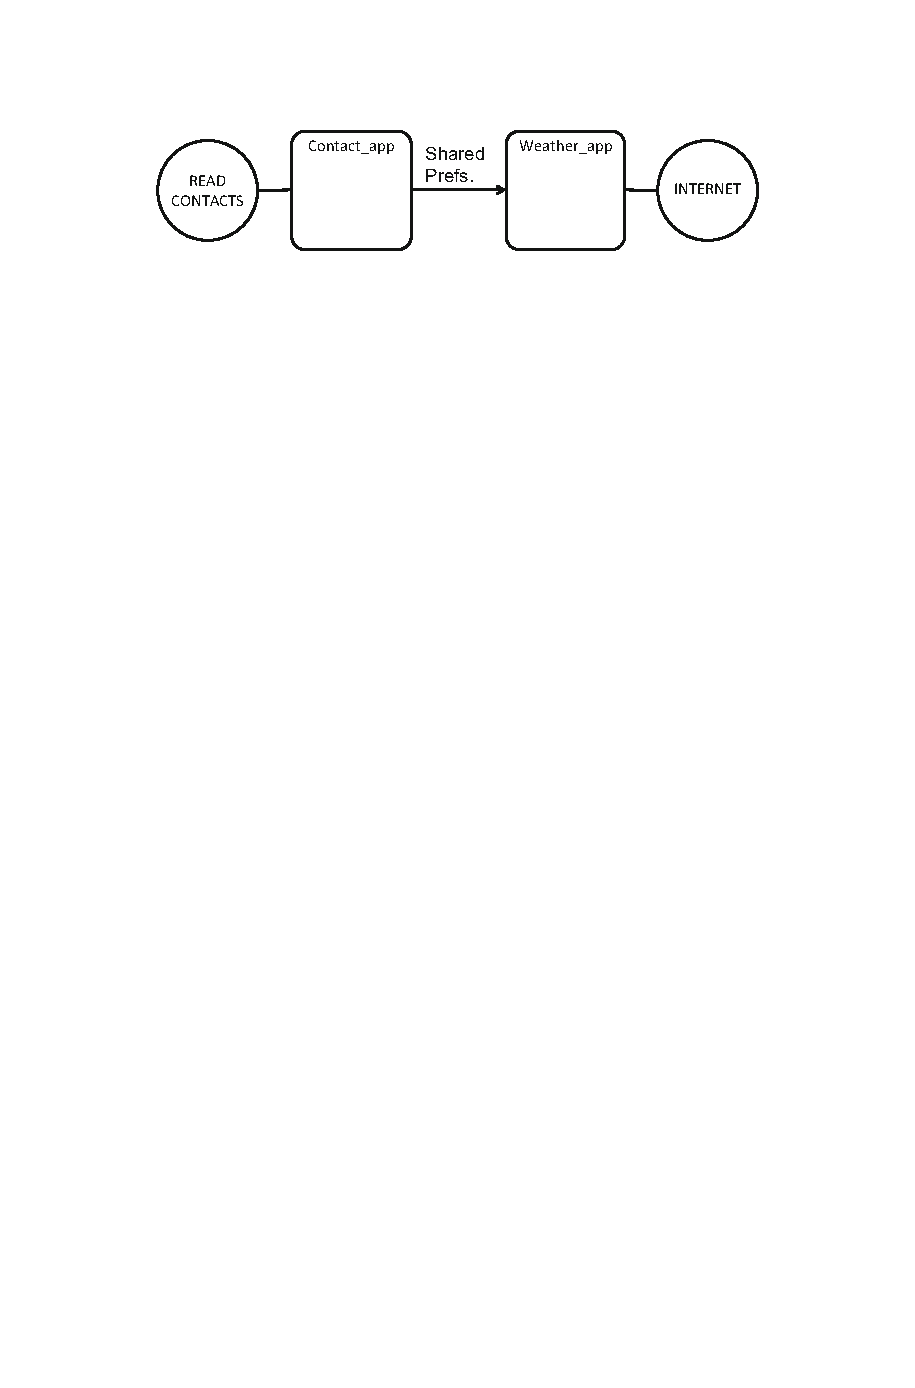
\includegraphics[width=\textwidth]{graphics/CollusionExample}
  \caption{Collusion}
  \label{fig:collusionExample}
\end{figure}

Here two applications are colluding to steal the user's contacts list.  One application has been granted permission to read the contacts list on the user's device but cannot transmit anything off the device.  It can, however, communicate with a second application that has access to the internet for receiving weather updates from an internet server.  These applications are able to combine their permissions to defeat the Android security system and steal information.  The contacts app can read the contact list and pass it to the weather app, then the weather app can transmit this information off the device to a hidden actor.

\qed
\end{myEx}

\noindent
A general description of collusion was put forward by As{\u a}voae et al. \cite{DetectingMaliciousCollusion}:\\

\begin{definition}
\label{def:Collusion}
There is a non-singleton set S of apps performing a threat such that:

\begin{itemize}

\item Each app in S contributes the execution of at least one action of the threat.
\item Each app in S communicates with at least one other app in S. 

\end{itemize}
\end{definition}

\noindent
The possibility of collusion was introduced as theoretical concept in 2011 by Schlegel et al. \cite{Soundcomber} where they developed a proof-of-concept called `Soundcomber'.  Soundcomber comprised of two applications communicating to steal the user's banking details.   Then, in 2017, collusion was confirmed in the wild thanks to the ACiD project \cite{ACiDProject}.

\subsection{Staging a Controlled Attack}
\label{sebsec:PerformingAControlledAttack}

In order to develop a means to detect collusion, we must have the ability to perform an attack at will and demonstrate that our countermeasures are able to recognise the attack.  The example in figure \ref{fig:collusionExample} provides us with the activities that constitute a threat to steal a users contacts list:

\begin{enumerate}
\item Application A reads the contacts list
\item Application A sends the contact list to application B.
\item Application B receives the contact list from application A.
\item Application B publishes the contact list
\end{enumerate}

We can see that applications A and B are attacking the system in a way that follows the definition \ref{def:Collusion} of collusion:  Two applications are involved, each application performs two actions from the threat, and each application is involved in communication with another.  Using that example to provide a collusion stimulus, we will produce two applications that carry out the attack described.  Details of the applications are left to section \ref{subsec:RHPracticalPerformanceAnalysisEnvironment} in the contribution, where we build a test environment.

%The Android security model guards against most attacks but cannot recognise collusion as a novel type of malware.  As such, colluding applications circumvent Android security.

%We demonstrate that colluding applications circumvent the security model.

%We examine how the Android security model guards against most attacks, but can be circumvented by colluding applications.\\
